\begin{comment}
2.1.3 Management Summary und Web-Publikation
Das Management Summary soll 2-5 Seiten umfassen sowie eine bis zwei Figuren enthalten. Es richtet sich an den „gebildete Laien“ auf dem Gebiet und beschreibt daher in erster Linie die (neuen und eigenen) Ergebnisse und Resultate der Arbeit. Die Sprache soll knapp, klar und stark untergliedert sein.
Grundlage für das Management Summary kann der Broschüren-Eintrag sein, den die Abteilung bei Diplomarbeiten jeweils früh verlangt, um eine Broschüre zu drucken. Das Management Summary dient als Vorlage für eine allfällige Web-Publikation.
Das Abstract und das Management Summary werden - zeitlich gesehen - gegen Schluss der Arbeit geschrieben und bilden zusammen mit den Schlussfolgerungen im technischen Bericht den am häufigsten gelesenen Teil der Arbeit. Diese Dokumente sollen daher am Sorgfältigsten ausgearbeitet sein.
Die folgenden Stichworte sollen die typische Struktur illustrieren, wobei die genaue Ausführung jeweils auf die spezifischen Bedürfnisse und Randbedingungen eines Projekts anzupassen ist. Diese Struktur kann auch für die Präsentation der Arbeit als "Richtschnur" dienen.
1. Ausgangslage
Warum machen wir das Projekt?
Welche Ziele wurden gesteckt (Kann-Ziele, Muss-Ziele)
Was machen andere / welche ähnlichen Arbeiten gibt es zum Thema?
Vorgehen: Was wurde gemacht? In welchen Teilschritten?
Risiken der Arbeit?
Wer war involviert (Durchführung, Entscheide usw.)?
Was konnte von anderen verwendet werden?
2. Ergebnisse
Was ist das Resultat?
Bewertung der Resultate, was ist Neuartig an der Arbeit?
Zielerreichung bezüglich Kann-/Muss-Zielen
Abweichungen (positiv und negativ) und kurze Begründung dafür
(Externe) Kosten der Arbeit?
Was ist der Nutzen (quantifizierbar/nicht quantifizierbar)?
3. Ausblick
Was hat man mit Durchführung des Projekts gelernt?
Verbleibende Probleme, (zukünftige) Gegenmassnahmen bez. Risiken
Was würde man anders machen, was ist weiter zu tun

Überschriften (Unterkapitel) ohne Nummerierung einsetzen!
\end{comment}


\phantomsection
\addcontentsline{toc}{chapter}{Management Summary}

\chapter*{Management Summary}
\glsresetall

\section*{Ausgangslage}

Den Schweizer Behörden steht frei, welche Software-Systeme sie einsetzen, um mit Geo-Daten zu arbeiten. Dies führt dazu, dass eine Vielzahl an Systemen eingesetzt und der Datenaustausch massiv erschwert wird. Es wurde versucht, dieses Problem mit dem Datenaustausch per \gls{interlis} zu lösen. Aufgrund mangelndert Unterstützung seitens der Software-Hersteller muss die Konvertierung in dieses Format jedoch nach wie vor von den am Austausch beteiligten Stellen selbst vorgenommen werden.

Dies bringt beachtlichen technischen und betrieblichen Aufwand mit sich.

\section*{Ziele}

Diese Arbeit hat als Ziel das Erstellen eines Prototypen für eine Plattform, welche
\begin{itemize}
\item diverse Daten-Formate lesen und schreiben kann, so dass ein Benutzer sich um die Daten kümmern kann, statt sich mit Formaten befassen zu müssen
\item fortgeschrittenen Benutzern erlaubt, neue Sichten oder Transformationen für bereitgestellte Daten zu erstellen, welche andere Benutzer dann weiter verwenden können
\item Benutzern ermöglicht, Daten öffentlich anzubieten.
\end{itemize}

Für das reine Anbieten von Daten existieren bereits gute Lösungen (siehe \cref{sec:tb:state-of-the-art}). Daher lag der Fokus auf der Unterstützung von Transformationen und verschiedenen Formaten.

\section*{Ergebnisse}
Im Rahmen der Arbeit wurde mit \acf{odh} eine moderne Web-Applikation erstellt.

\subsection*{Formate}
Benutzer können Daten mit anderen Benutzern teilen ohne sich um Format-Details kümmern zu müssen. Unterstützt werden Formate wie CSV, Excel, JSON aber auch Geo-Formate wie GeoJSON, GML, Interlis 1 sowie Daten aus \gls{wfs}-Endpunkten.

Weiterhin besteht die Möglichkeit, aus einer Analyse der bereit gestellten Daten ein Interlis 1-Modell zu erstellen.

\subsection*{Transformationen}
Mit Hilfe eines Assistenten können Benutzer sich eine einfach Transformation zusammenklicken und anderen Benutzern zur Verfügung stellen. 

Für Experten steht mit \gls{odhql} eine an \gls{sql} angelehnte Abfrage-Sprache bereit, welche auch komplexe Abfragen ermöglicht.

\begin{figure}[H]
    \centering
    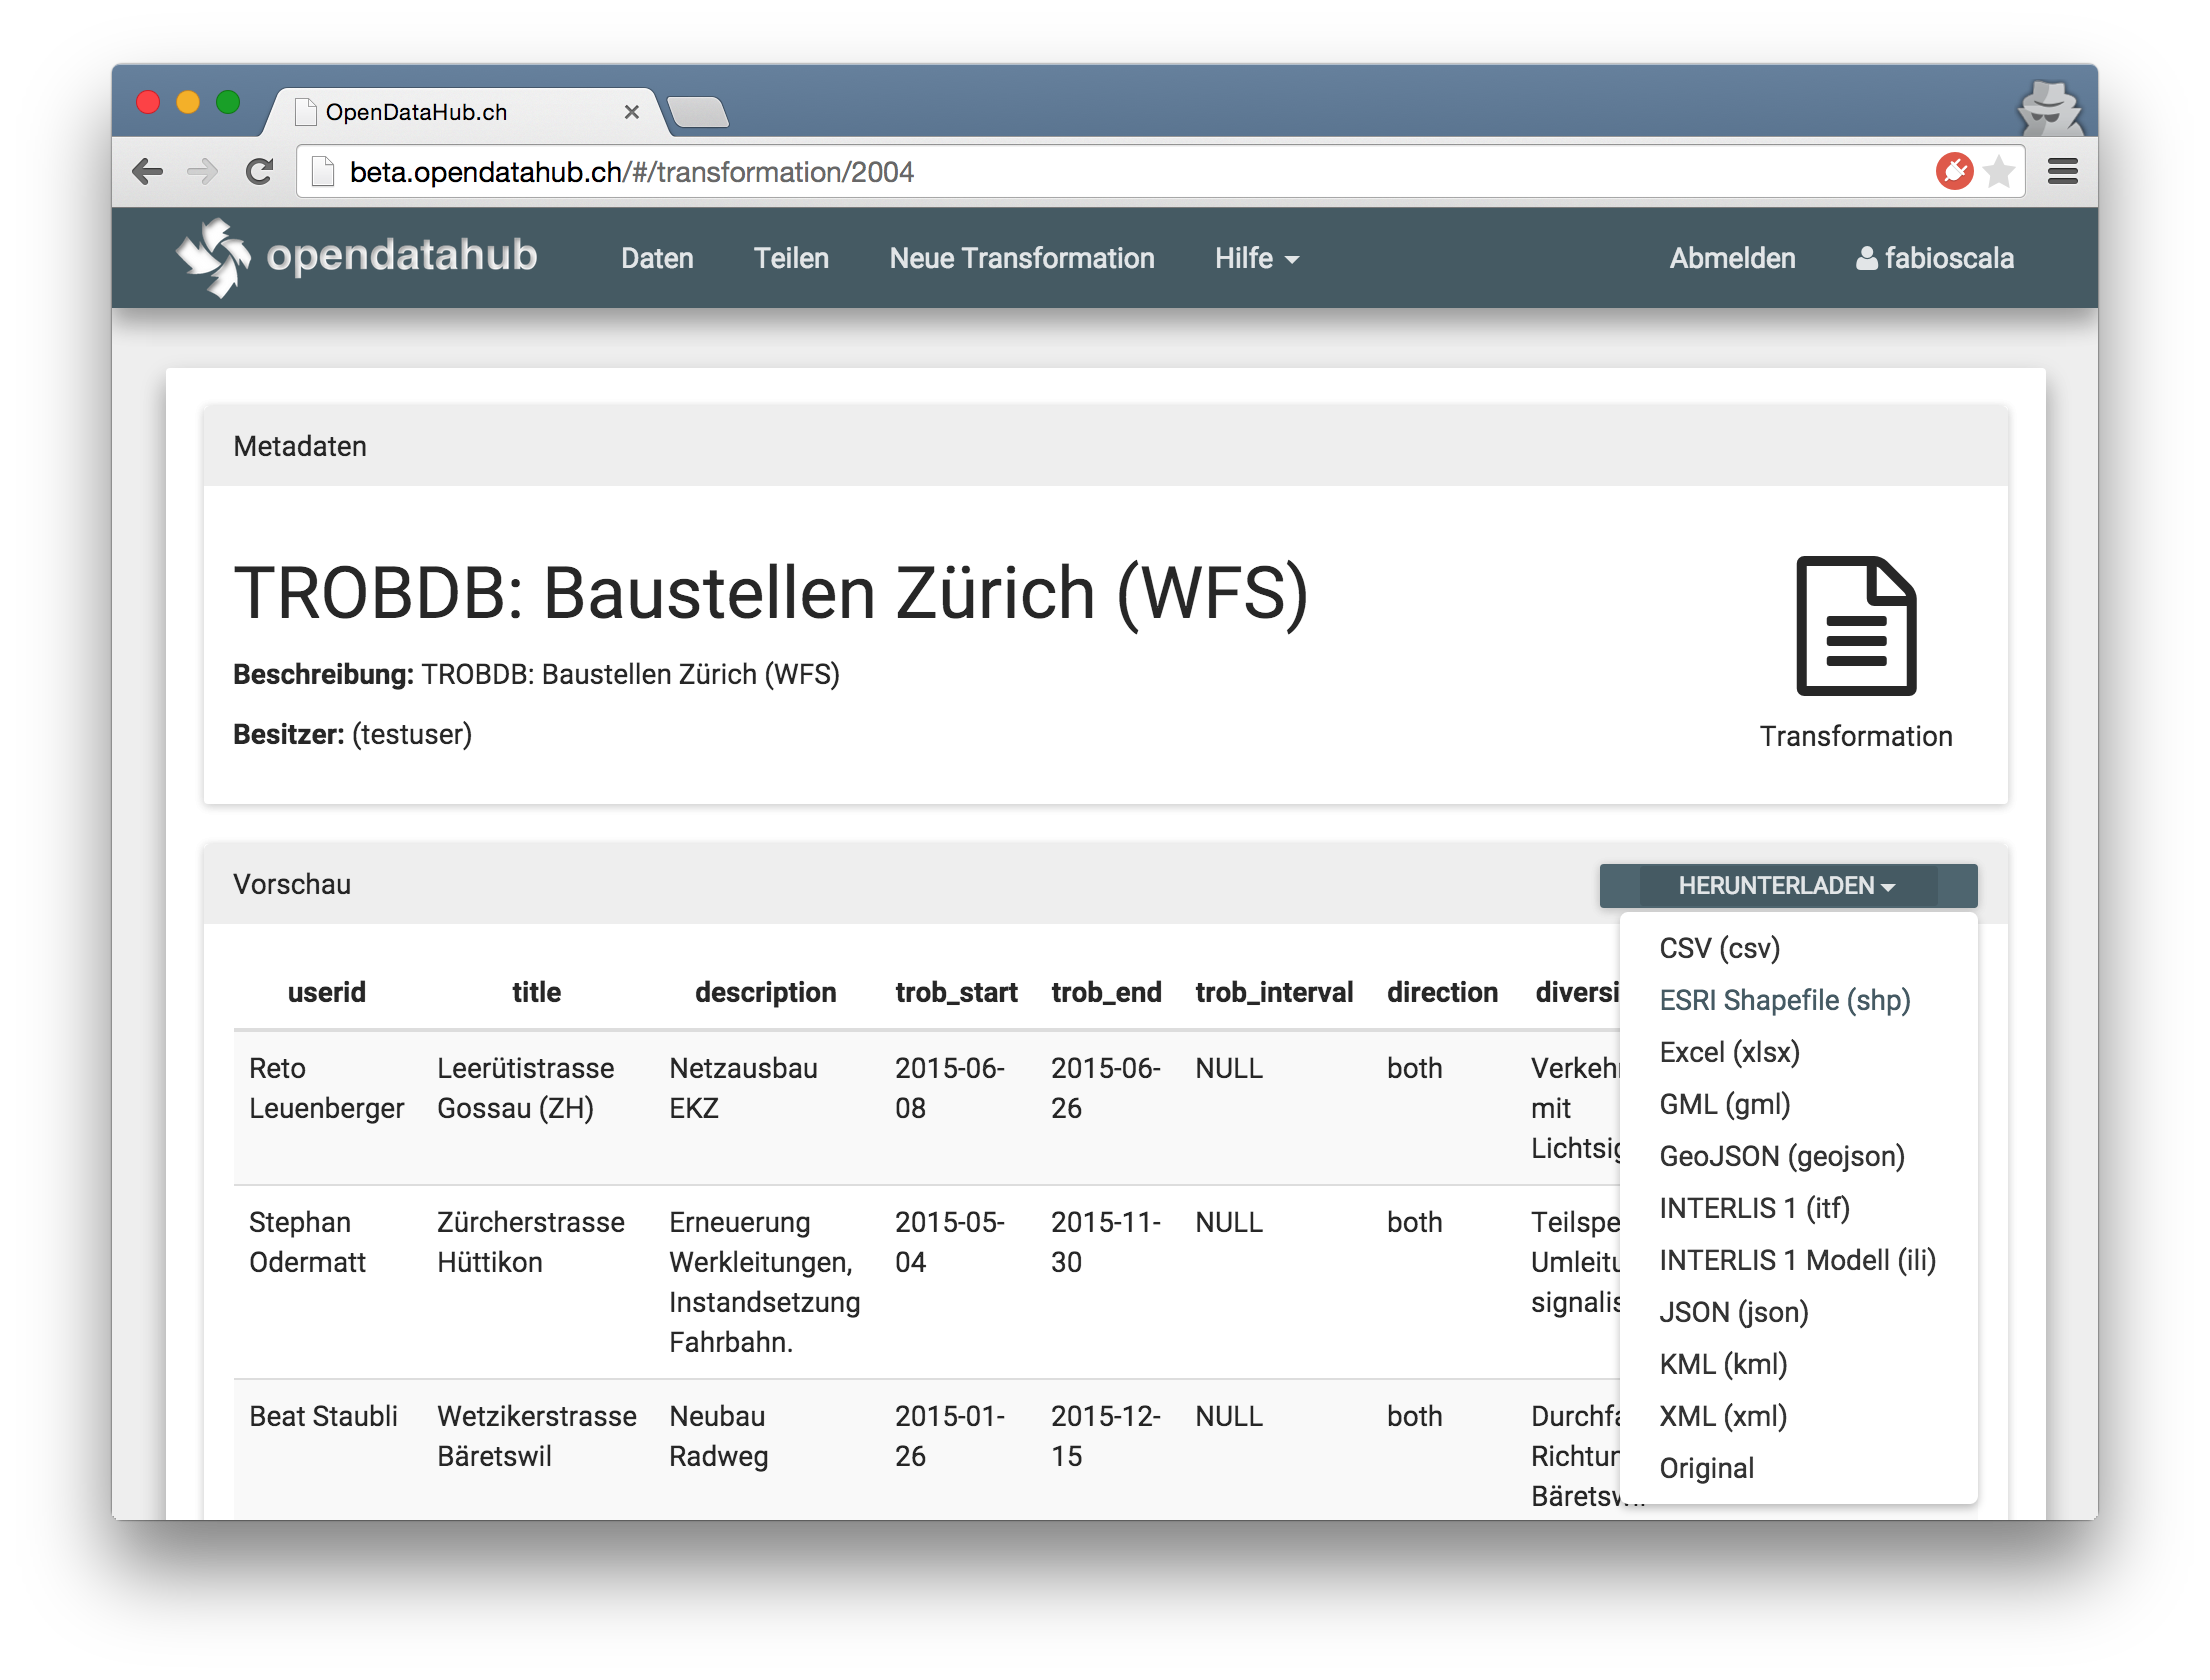
\includegraphics[width=2\linewidth/3]{fig/transformation-detail}
    \caption*{Resultat einer Transformation}
\end{figure}

Die Resultate von Transformationen können wie alle anderen Daten auch in beliebigen Formaten bezogen werden.

\subsection*{Erweiterung}
Neue Formate sowie Funktionen für die Abfrage-Sprache können mit relativ wenig Aufwand hinzugefügt werden.

\section*{Ausblick}
Für die Weiterentwicklung von \acs{odh} besteht eine Vielzahl an Möglichkeiten. Hier eine Auswahl:
\begin{itemize}
\item Wechsel auf neue Versionen der zur Format-Unterstützung verwendeten Bibliotheken.
\item Erweiterung der Web-Applikation, evtl. Integration mit bereits vorhander Software.
\item Ausbau des Transformations-Assistenten um weitere Features.
\item Unterstützung für weitere Formate.
\end{itemize}
